\documentclass[11pt,a4paper]{article}
\usepackage[a4paper,top=14mm,bottom=14mm,left=15mm,right=15mm,headsep=5mm,footskip=6mm]{geometry}
\usepackage[T1]{fontenc}
\usepackage{libertinus}
\usepackage[final]{microtype}
\usepackage{amsmath,amssymb,mathtools,bm}
\usepackage{xcolor}
\usepackage{multicol,booktabs,tabularx,array,enumitem}
\usepackage{tikz}
\usetikzlibrary{arrows.meta,positioning,calc}
\usepackage[most]{tcolorbox}
\usepackage{fancyhdr}
\usepackage{hyperref}
\hypersetup{colorlinks=true,linkcolor=teal!45!black,urlcolor=teal!45!black,pdftitle={PHYS7045: Five-Page Formula and Method Sheet},pdfauthor={Quantum Technologies revision reference}}
\definecolor{ink}{HTML}{263746}
\definecolor{accent}{HTML}{11677A}
\definecolor{muted}{HTML}{5A6977}
\definecolor{soft}{HTML}{F0F5F7}
\definecolor{warm}{HTML}{F9F6EE}
\AtBeginDocument{\color{ink}}
\setlength{\parindent}{0pt}
\setlength{\parskip}{2.2pt plus 0.3pt minus .3pt}
\setlength{\columnsep}{7mm}
\setlength{\columnseprule}{0.25pt}
\setlength{\multicolsep}{2pt}
\setlength{\emergencystretch}{2em}
\setlist[enumerate]{leftmargin=*,topsep=2pt,itemsep=1pt,parsep=0pt}
\setlist[itemize]{leftmargin=*,topsep=2pt,itemsep=.6pt,parsep=0pt}
\newcommand{\ket}[1]{\left\lvert #1\right\rangle}
\newcommand{\bra}[1]{\left\langle #1\right\rvert}
\newcommand{\braket}[2]{\left\langle #1\middle|#2\right\rangle}
\newcommand{\I}{\mathbb I}
\newcommand{\Tr}{\operatorname{Tr}}
\newcommand{\D}{\mathcal D}
\newcommand{\ee}{\mathrm e}
\newcommand{\dd}{\mathrm d}
\newcommand{\synd}{\operatorname{syn}}
\newcommand{\wt}{\operatorname{wt}}
\newcommand{\R}{\mathcal R}
\newcommand{\smallbox}[1]{\begin{tcolorbox}[colback=soft,colframe=accent!40!white,boxrule=0.4pt,arc=1mm,left=1.2mm,right=1.2mm,top=.7mm,bottom=.7mm,before skip=2pt,after skip=2pt]\footnotesize #1\end{tcolorbox}}
\newcommand{\caution}[1]{\begin{tcolorbox}[colback=warm,colframe=black!17,boxrule=0.35pt,arc=1mm,left=1.2mm,right=1.2mm,top=.7mm,bottom=.7mm,before skip=2pt,after skip=2pt]\footnotesize #1\end{tcolorbox}}
\newcommand{\topic}[1]{\par\vspace{3pt}{\color{accent}\bfseries #1}\par\vspace{-1pt}}
\newcommand{\paper}[1]{{\color{muted}\footnotesize\emph{#1}}}
\newcommand{\pagetitle}[2]{\noindent{\color{accent}\fontsize{16}{18}\selectfont\bfseries #1}\hfill{\footnotesize\color{muted}#2}\par\vspace{1pt}\hrule\vspace{4pt}}
\pagestyle{fancy}
\fancyhf{}
\fancyhead[L]{\footnotesize\color{muted}PHYS7045 \textbar\ Exam method sheet}
\fancyhead[R]{\footnotesize\color{muted}Formula \textrightarrow\ method \textrightarrow\ check}
\fancyfoot[L]{\scriptsize\color{muted}2023--2025 papers + 2026 assignment types}
\fancyfoot[R]{\footnotesize\bfseries\color{accent}\thepage\ / 5}
\renewcommand{\headrulewidth}{0.2pt}
\renewcommand{\footrulewidth}{0pt}
\begin{document}
\pagetitle{1. States, matrices and entangling gates}{2023 Q3; all pulse and protocol questions}
\smallbox{\textbf{Universal exam procedure:} (1) State the basis and qubit ordering; (2) identify the physical subspace or operator; (3) apply it to each relevant basis input, preserving relative phases; (4) normalise or assemble the matrix; (5) check unitarity, probabilities and whether any ancilla returns to its initial state.}
\begin{multicols}{2}
\topic{A. Translate a Hamiltonian into a gate}
For a time-independent closed-system Hamiltonian,
\[U(t)=\ee^{-iHt/\hbar}.\]
If $A^2=\I$ (a Pauli matrix or Pauli product),
\[\boxed{\ee^{-i\theta A}=\cos\theta\,\I-i\sin\theta\,A.}\]
\textbf{Method:} expand $H$; move any term proportional to $\I$ into a global phase; identify $A^2=\I$; substitute into the identity; \emph{apply to input states rather than guessing the gate}. Keep the global phase if asked for the exact unitary, omit it only when identifying physical gate action.

\topic{B. Worked pattern: the 2023 $YY$ Hamiltonian}
\paper{2023 Q3A1--2: $H=\frac{\hbar g}{2}(Y_1+Y_2)^2$.}
Since $Y_i^2=\I$ and $[Y_1,Y_2]=0$,
\[H=\hbar g(\I+Y\otimes Y),\]
\[U=\ee^{-igt}\{\cos(gt)\I-i\sin(gt)Y\otimes Y\}.\]
The overall $\ee^{-igt}$ is a global phase. Using $Y\ket0=i\ket1$,
\[U\ket{00}\sim\cos(gt)\ket{00}+i\sin(gt)\ket{11}.\]
\textbf{Bell-state condition:} equal amplitudes $\Rightarrow\cos(gt)=\sin(gt)$, so
\[\boxed{t_{\rm ent}=\frac{\pi}{4g},\quad \ket\psi\sim\frac{\ket{00}+i\ket{11}}{\sqrt2}.}\]
\textbf{Test:} the reduced state of either qubit is $\I/2$, confirming maximal entanglement.

\topic{C. Convert an entangler to CNOT}
\paper{2023 Q3B; 2025 Q2A5.}
Use local rotations to change the Pauli axis, then transform CZ into CNOT:
\[R_x(\pi/2)Y R_x(-\pi/2)=Z,\]
\[\ee^{-i\pi YY/4}\xrightarrow{\ R_x\otimes R_x\ }\ee^{-i\pi ZZ/4}.\]
For $S=\operatorname{diag}(1,i)$,
\[(S^\dagger\!\otimes S^\dagger)\ee^{-i\pi ZZ/4}=\ee^{-i\pi/4}\mathrm{CZ},\]
\[\boxed{\mathrm{CNOT}_{A\to B}=(\I\otimes H)\mathrm{CZ}(\I\otimes H).}\]
\textbf{Procedure:} show axes $YY\to ZZ$; remove local phase gates; put Hadamards around \emph{target} to turn controlled phase into controlled flip.

\columnbreak
\topic{D. Qubit rotations and pulse areas}
For a resonantly driven qubit,
\[H=\frac{\hbar\Omega}{2}\,\hat{\bm n}\!\cdot\!\bm\sigma,\qquad \theta=\Omega t,\]
\[R_{\hat{\bm n}}(\theta)=\cos\tfrac\theta2\I-i\sin\tfrac\theta2\hat{\bm n}\!\cdot\!\bm\sigma.\]
A $\pi$ pulse transfers population in the addressed two-state subspace (phase $-i$ for a standard $x$ pulse); a $2\pi$ pulse returns the state with phase $-1$. For a general drive
\[H_{\rm rot}=\tfrac{\hbar}{2}(\Omega X+\delta Z),\quad \Omega_R=\sqrt{\Omega^2+\delta^2}.\]
\textbf{Watch the factor of two:} if $H=\hbar t_c X$ (rather than $\hbar\Omega X/2$), then $\theta=2t_ct$.

\topic{E. Work with qubit states and density matrices}
\[\ket\psi=\cos\tfrac\theta2\ket0+\ee^{i\phi}\sin\tfrac\theta2\ket1,\]
\[\rho=\tfrac12(\I+r_xX+r_yY+r_zZ)\]
\[\phantom{\rho}=\tfrac12\begin{pmatrix}1+r_z&r_x-ir_y\\r_x+ir_y&1-r_z\end{pmatrix}.\]
Reading a matrix: diagonal $\to$ populations; off-diagonals $\to$ coherence. Bloch components $r_j=\Tr(\rho\sigma_j)$; pure states $|\bm r|=1$, mixed states $|\bm r|<1$.
\[\Tr(\rho^2)=\tfrac12(1+|\bm r|^2),\quad \langle A\rangle=\Tr(\rho A).\]
For a bipartite state, discard an inaccessible system by $\rho_B=\Tr_A\rho_{AB}$. For a Bell state, $\rho_{AB}$ is pure but $\rho_A=\rho_B=\I/2$.

\topic{F. Recognise the physical answer being sought}
\begin{tabularx}{\linewidth}{@{}p{.36\linewidth}X@{}}\toprule
Question wording & What to show \\ \midrule
``Determine unitary'' & $U=\exp(-iHt/\hbar)$, basis, phases \\
``Maximally entangled'' & two equal Schmidt coefficients \\
``Gate matrix'' & transform \emph{all} basis vectors; outputs are columns \\
``CNOT from CZ'' & Hadamards on the target \\
``Fastest gate'' & maximise available angular frequency; $t=\theta/\Omega_R$ \\
\bottomrule\end{tabularx}
\caution{\textbf{Common mistake:} $Y\otimes Y$ is not $Y\otimes\I+\I\otimes Y$. Distinguish the Hamiltonian's stated Pauli product from its square and include all global factors in an exact exponential.}
\end{multicols}
\clearpage
\pagetitle{2. Stabiliser codes: solve any unfamiliar code}{2023 Q2; 2024 Q1; 2025 Q1}
\smallbox{\textbf{Six-step workflow for every past-paper QEC problem:} Check generators commute $\to$ calculate $k$ $\to$ compute syndromes $\to$ test correctability (including degeneracy) $\to$ find $X_L,Z_L$ $\to$ prove the minimum distance $d$. This is a method, not a code to memorise.}
\begin{multicols}{2}
\topic{A. Commutation without large matrices}
At a qubit position, distinct nonidentity Paulis ($X/Y$, $X/Z$, $Y/Z$) \emph{anticommute}; equal Paulis or any $I$ commute. Two tensor-product Paulis obey
\[PQ=(-1)^mQP,\]
where $m$ is the \emph{number of anticommuting positions}. Even $m\to$ commute; odd $m\to$ anticommute.
\[\begin{array}{@{}lcl@{}}ZIZ &\text{vs}& XIY:\ m=2\;\checkmark\\ZIZ &\text{vs}& XII:\ m=1\;\times\end{array}\]
For $n$ qubits and $r$ independent, commuting generators (with $-I$ excluded):
\[\boxed{k=n-r.}\]
\textbf{Why?} Each independent $+1$ stabiliser halves the $2^n$-dimensional Hilbert space; the code has dimension $2^{n-r}$.

\topic{B. Syndrome table, one physical error at a time}
For an error $E$, define $b_i=0$ if $[E,S_i]=0$ and $b_i=1$ if $\{E,S_i\}=0$. The measured eigenvalue is $(-1)^{b_i}$. \emph{Calculate each $b_i$ by counting overlaps.}

\textbf{Example:} $S_1=Z_1Z_2$, $S_2=Z_2Z_3$ for the three-qubit bit-flip code:
\begin{center}\footnotesize
\begin{tabular}{@{}cccc@{}}\toprule
$E$ & $S_1$ & $S_2$ & syndrome $b_1b_2$ \\ \midrule
$I$ & $+$ & $+$ & $00$\\
$X_1$ & $-$ & $+$ & $10$\\
$X_2$ & $-$ & $-$ & $11$\\
$X_3$ & $+$ & $-$ & $01$\\
$Z_1$ & $+$ & $+$ & $00$\\
\bottomrule\end{tabular}
\end{center}
The two checks identify any \emph{single bit flip} but cannot detect $Z_1$: this is not a general one-error quantum code.

\topic{C. Detection vs correction; resolve collisions}
\textbf{Detect} an error if its syndrome is nonzero (or it is a stabiliser acting trivially). To \textbf{correct an entire set} $\{E_a\}$, comparing two possible errors matters:
\begin{enumerate}
\item Different syndromes $\to$ decoder can distinguish them.
\item Same syndrome $\to$ calculate $E_a^\dagger E_b$.
\item If $E_a^\dagger E_b\in\mathcal S$, the collision is \emph{harmless degeneracy}. If it lies in $\mathcal N(\mathcal S)\setminus\mathcal S$, it is an uncorrectable logical ambiguity.
\end{enumerate}
General condition: $PE_a^\dagger E_bP=c_{ab}P$, with $P$ the code-space projector.

\columnbreak
\topic{D. Two actual collisions to recognise}
\textbf{2023 Q2:} $\synd(Z_1)=\synd(Z_3)$, but $Z_1Z_3=S_1$ (a stabiliser). Either correction has the same logical action: \emph{correctable}.

\textbf{2024 Q1:} $\synd(X_1)=\synd(X_2)$, but $X_1X_2=X_L$ is a nontrivial logical operation. Wrong recovery changes the encoded state: \emph{not fully correctable}.

\topic{E. Find logical Paulis and code distance}
Candidate logical $L$ must commute with \emph{every} stabiliser but not belong to $\mathcal S$. Select $X_L,Z_L$ with
\[[L,S_i]=0,\quad X_LZ_L=-Z_LX_L.\]
Multiplication by a stabiliser gives an equivalent logical representative. Weight $\wt(L)$ counts non-$I$ factors. The distance is
\[\boxed{d=\min_{L\in\mathcal N(\mathcal S)\setminus\mathcal S}\wt(L),\qquad t=\left\lfloor\frac{d-1}{2}\right\rfloor.}\]
\textbf{To prove $d$:} (1) show a particular logical operator of weight $w$ $\Rightarrow d\le w$; (2) rule out all lower-weight nontrivial logicals (often by showing correction of all one-qubit Pauli errors) $\Rightarrow d\ge w$.

\topic{F. Historical code results (reusable checks)}
\begin{center}\footnotesize
\begin{tabular}{@{}llll@{}}\toprule
Paper&$[[n,k,d]]$&$X_L$ example&$Z_L$ example\\\midrule
2023&$[[6,1,3]]$&$XZXZII$&$XYYXII$\\
2024&$[[5,1,2]]$&$XXIII$&$ZIIZI$\\
2025&$[[9,1,3]]$&$Z_1Z_4Z_7$&$X_1X_2X_3$\\
\bottomrule\end{tabular}
\end{center}
\textbf{2025 Shor-type code:} six $Z$-pair checks identify a bit flip within a 3-qubit block. Two six-body $X$ checks locate a phase-flip \emph{block}. Different $Z$ errors within the same block differ by stabilisers, so they are equivalent and correctable. $Y$ triggers both patterns.

\topic{G. CSS and transversal-gate cue}
In CSS codes, \emph{$Z$ checks detect $X$ errors}, while \emph{$X$ checks detect $Z$ errors}. The Steane code is $[[7,1,3]]$; it corrects one arbitrary physical Pauli error. A transversal CNOT is formed by applying physical CNOTs between \emph{corresponding} qubits of two blocks; show its action on $X_L,Z_L$ to establish the logical gate.
\caution{\textbf{Exam trap:} all 15 weight-one Paulis can have nonzero syndromes and the code can still fail to \emph{correct} one error. The 2024 code is precisely this example: $d=2$, so $t=0$ for arbitrary noise.}
\end{multicols}
\clearpage
\pagetitle{3. Physical gates: trapped ions and Rydberg atoms}{2023 Q1; 2024 Q3; 2025 Q2}
\smallbox{\textbf{Physical-gate recipe:} State which electronic/motional transition is resonant; identify dark (uncoupled) branches; track each basis state through \emph{each} pulse; retain factors $-i$ and $-1$; check the bus/auxiliary system is restored; read off the computational unitary.}
\begin{multicols}{2}
\topic{A. Ions: sidebands and phonon factors}
Write the state as $\ket{\text{ion},n}$, including phonon number $n$.
\begin{center}\footnotesize
\begin{tabular}{@{}lll@{}}\toprule
Laser&Transition&Rate\\\midrule
Carrier&$\ket{g,n}\leftrightarrow\ket{e,n}$&$\Omega$\\
Red&$\ket{g,n}\leftrightarrow\ket{e,n-1}$&$\eta\Omega\sqrt{n}$\\
Blue&$\ket{g,n}\leftrightarrow\ket{e,n+1}$&$\eta\Omega\sqrt{n+1}$\\
\bottomrule\end{tabular}
\end{center}
$a\ket n=\sqrt n\ket{n-1}$; $a^\dagger\ket n=\sqrt{n+1}\ket{n+1}$. Therefore $\ket{g,0}$ is \emph{dark to red-sideband excitation}, but $\ket{e,0}\leftrightarrow\ket{g,1}$ couples.

\topic{B. 2025 Q2: $\pi_A\!\to2\pi_B\!\to\pi_A$}
Let $\ket e=\ket1$, $\ket g=\ket0$, initial $n=0$. Ion $A$: red sideband $g\leftrightarrow e$; ion $B$: auxiliary $g\leftrightarrow a$. The active $\pi$ step multiplies by $-i$; the active $2\pi$ cycle multiplies by $-1$.
\begin{center}\footnotesize\renewcommand{\arraystretch}{1.14}
\begin{tabular}{@{}llll@{}}\toprule
Input&after $\pi_A$&after $2\pi_B$&final $\pi_A$\\\midrule
$gg,0$&$gg,0$&$gg,0$&$gg,0$\\
$ge,0$&$ge,0$&$ge,0$&$ge,0$\\
$eg,0$&$-i gg,1$&$+i gg,1$&$+eg,0$\\
$ee,0$&$-i ge,1$&$-i ge,1$&$-ee,0$\\
\bottomrule\end{tabular}
\end{center}
\[\boxed{U=\operatorname{diag}(1,1,1,-1)=\mathrm{CZ}.}\]
\textbf{Method:} the $B$ $2\pi$ pulse is active \emph{only when} a phonon exists and $B=g$. Every branch ends with $n=0$; put its final phase on the diagonal.

\textbf{Extension:} 2025 Q2B, a CCZ uses five pulses $\pi_A\to\pi_B\to2\pi_C\to\pi_B\to\pi_A$, so only $\ket{111}$ acquires $-1$. A Toffoli is $H$ on the target before/after CCZ.

\topic{C. 2023 Q1: the M\o lmer--S\o rensen mechanism}
Two virtual paths exchange phonons with opposite detunings $\pm\delta$. Using the problem's second-order rate $\Omega_{2\gamma}=\Omega_1\Omega_2/(2\delta)$ and summing both ion orderings,
\[\Omega_{n+1}=\frac{\eta^2\Omega_r\Omega_b(n+1)}{\delta},\quad
\Omega_{n}=-\frac{\eta^2\Omega_r\Omega_b n}{\delta}.\]
\[\boxed{\Omega_{\rm eff}=|\Omega_{n+1}+\Omega_n|=\frac{\eta^2|\Omega_r\Omega_b|}{|\delta|}.}\]
The $n$-dependent pieces cancel: $(n+1)-n=1$. A Bell state from $\ket{gg}$ requires a $\pi/2$ \emph{effective} pulse:
\[\boxed{t_{\rm Bell}=\pi/(2\Omega_{\rm eff}).}\]
This relies on virtual intermediate states ($|\delta|\gg$ sideband coupling), correct relative detuning signs, and laser-phase calibration.

\columnbreak
\topic{D. 2024 Q3: simultaneous Rydberg drives}
\emph{Levels:} the control has $\Omega_1:\ket0\leftrightarrow\ket r$; the target also receives $\Omega_2:\ket1\leftrightarrow\ket r$. Simultaneous two-colour target driving can swap $\ket0\leftrightarrow\ket1$ via $\ket r$ \emph{unless} the control is Rydberg excited.

\begin{center}
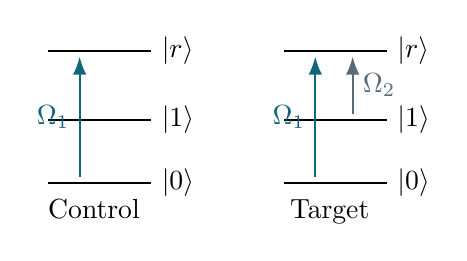
\begin{tikzpicture}[>=Latex,scale=.73]
 \foreach \x/\lab in {0/Control,4.1/Target}{
  \draw[thick] (\x,0)--(\x+1.8,0) node[right] {$\ket0$};
  \draw[thick] (\x,1.1)--(\x+1.8,1.1) node[right] {$\ket1$};
  \draw[thick] (\x,2.3)--(\x+1.8,2.3) node[right] {$\ket r$};
  \node[below] at (\x+.8,-.12) {\lab};
  \draw[->,thick,accent] (\x+.55,.1)--(\x+.55,2.2) node[midway,left] {$\Omega_1$};}
 \draw[->,thick,muted] (5.3,1.2)--(5.3,2.2) node[midway,right] {$\Omega_2$};
\end{tikzpicture}
\end{center}
\textbf{Blockade:} $|U_{rr}|/\hbar\gg\Omega_1,\Omega_2$ shifts the target's intermediate level off resonance when the control is $\ket r$.

\begin{center}\footnotesize
\begin{tabular}{@{}ccc@{}}\toprule
Input&Target flip?&Output (ignoring phases)\\\midrule
$\ket{1_c0_t}$&yes&$\ket{1_c1_t}$\\
$\ket{1_c1_t}$&yes&$\ket{1_c0_t}$\\
$\ket{0_c0_t}$&blocked&$\ket{0_c0_t}$\\
$\ket{0_c1_t}$&blocked&$\ket{0_c1_t}$\\
\bottomrule\end{tabular}
\end{center}
\textbf{Pulse method:} engineer a \emph{closed} $2\pi$ control excursion and a target \emph{effective} $\pi$ bit flip in the unblocked branch. For equal resonant target couplings, the physical 3-level \emph{bright-state} cycle is $2\pi$ to implement the swap ($-X$), not a naive direct two-level $\pi$ pulse. Exact durations need the coupling ratio/detuning/envelopes.

\topic{E. Extend the geometry to Toffoli}
Place controls at opposite sides of a central target ($c_1-t-c_2$) so each control can blockade the target, but controls do not mutually blockade. Only $c_1=c_2=1$ leaves the target unblocked:
\[\ket{c_1c_2t}\mapsto\ket{c_1c_2,\ t\oplus(c_1c_2)}.\]
\textbf{Check:} identify any local phases from completed Rydberg cycles and compensate if the task requires the \emph{exact} gate, rather than the classical truth table.
\caution{\textbf{Key distinction:} MS motion is approximately \emph{virtually} excited and need not start in $n=0$; the 2025 resonant three-pulse gate explicitly uses a real phonon and starts in the motional ground state.}
\end{multicols}
\clearpage
\pagetitle{4. Photons, teleportation and state preparation}{2024 Q2; 2025 Q3; 2026 HOM}
\smallbox{\textbf{Photonics rule:} choose the encoding first. \emph{Dual-rail:} one photon distributed between two modes, $\ket{0_L}=\ket{1,0}$ and $\ket{1_L}=\ket{0,1}$. \emph{Single-rail:} vacuum $\ket0$ vs one photon $\ket1$ in one mode. The 2024 paper switches encoding between its two parts.}
\begin{multicols}{2}
\topic{A. Beam-splitter matrix from creation operators}
\paper{2024 Q2A.} If the given mapping is
\begin{align*}
a^\dagger&\mapsto a^\dagger\cos\theta+b^\dagger\ee^{i\phi}\sin\theta,\\
b^\dagger&\mapsto b^\dagger\cos\theta-a^\dagger\ee^{-i\phi}\sin\theta,
\end{align*}
\textbf{apply to $a^\dagger\ket{\rm vac}$ and $b^\dagger\ket{\rm vac}$.} Place resulting coefficients as columns:
\[B(\theta,\phi)=\begin{pmatrix}\cos\theta&-\ee^{-i\phi}\sin\theta\\\ee^{i\phi}\sin\theta&\cos\theta\end{pmatrix}.\]
For $\theta=\pi/4$, $\phi=0$: $B=HZ$, so an \emph{input $\pi$ phase shift} on the second rail gives exactly
\[\boxed{H=B(\pi/4,0)Z.}\]
Check matrix column order and phase convention: a bare beam splitter of this form has equal diagonal entries, so cannot equal the standard $H$ alone.

\topic{B. Hong--Ou--Mandel: two identical photons}
For a balanced splitter in a convenient phase convention,
\[a^\dagger\mapsto(c^\dagger+d^\dagger)/\sqrt2,\quad
b^\dagger\mapsto(c^\dagger-d^\dagger)/\sqrt2.\]
Apply \emph{both} operators to $\ket{1,1}=a^\dagger b^\dagger\ket{\rm vac}$:
\[\ket{1,1}\mapsto\frac{(c^\dagger)^2-(d^\dagger)^2}{2}\ket{\rm vac}=\frac{\ket{2,0}-\ket{0,2}}{\sqrt2}.\]
\textbf{Check:} no $\ket{1,1}$ coincidence term. The two alternatives cancel when photons are indistinguishable; distinguishability destroys that cancellation. Use $\ket{2,0}=(c^\dagger)^2\ket{\rm vac}/\sqrt2$ to get the factors right.

\topic{C. 2024 Q2B: heralded single-rail teleportation}
Input in mode 0: $\ket\psi_0=\alpha\ket0+\beta\ket1$; resource across modes 1--2:
\[\ket t_{12}=\frac{\ket{0,1}+\ket{1,0}}{\sqrt2}.\]
Expand $(\alpha\ket0+\beta\ket1)\otimes\ket t$. \textbf{Project first} onto $n_0+n_1=1$ at Alice's detectors. The unnormalised surviving state is
\[\ket{\Psi_1}=\frac{\alpha\ket{0,1}_{01}\ket0_2+\beta\ket{1,0}_{01}\ket1_2}{\sqrt2}.\]
$\Vert\Psi_1\Vert^2=(|\alpha|^2+|\beta|^2)/2=1/2$. After Alice's splitter, each one-click detector pattern has probability $1/4$:
\begin{center}\footnotesize
\begin{tabular}{@{}ccc@{}}\toprule
$(n_0,n_1)$&Bob's conditional state&Correction\\\midrule
$(0,1)$&$\alpha\ket0+\beta\ket1$&$I$\\
$(1,0)$&$\alpha\ket0-\beta\ket1$&$Z$\\
\bottomrule\end{tabular}
\end{center}
\[\boxed{P_{\rm success}=\tfrac14+\tfrac14=\tfrac12.}\]
Zero or two counts are failure events, not alternate recoveries.

\columnbreak
\topic{D. Standard qubit teleportation}
Alice possesses an \emph{unknown} $\ket\psi$ and her half of a Bell pair; Bob has the other half. Procedure:
\begin{enumerate}
\item Alice performs a Bell measurement on the unknown qubit and her resource qubit.
\item Send its \emph{two classical bits} to Bob.
\item Bob applies the corresponding $I,X,Z,XZ$ correction (depending on Bell convention).
\end{enumerate}
The input is consumed (no cloning). Bob's unconditioned state cannot reveal Alice's outcome: no superluminal signalling.

\topic{E. 2025 Q3: equatorial remote preparation}
\paper{State known to Alice, singlet shared with Bob.}
Target and axis are
\[\ket\beta=\frac{\ket0+\ee^{i\phi}\ket1}{\sqrt2},\quad \bm n=(-\sin\phi,\cos\phi,0).\]
Alice acts with $R_{\bm n}(\pi/2)$ then measures $Z$:
\[R=\frac1{\sqrt2}\begin{pmatrix}1&-\ee^{-i\phi}\\\ee^{i\phi}&1\end{pmatrix}.\]
Apply $(R\otimes I)$ to $\ket{\Psi^-}=(\ket{01}-\ket{10})/\sqrt2$; group by Alice's $\ket0,\ket1$ and normalise Bob's states:
\[\boxed{m=0:\ \ket\beta,\qquad m=1:\ Z\ket\beta}\]
(up to global phases; each probability $1/2$). Alice sends \emph{one bit}; Bob corrects with $Z^m$. Polarisation implementation: entangled-photon source $\to$ Alice waveplates $\to$ PBS and two detectors $\to$ classical bit $\to$ Bob phase plate.

\textbf{Arbitrary target} $\ket{\beta'}=\cos(\theta/2)\ket0+\ee^{i\phi}\sin(\theta/2)\ket1$: Alice also controls $\theta$ via waveplates. The other measurement outcome is orthogonal and \emph{cannot} be corrected by a single universal $Z$ for all $\theta,\phi$; accept a heralded $1/2$ branch or use more general feed-forward/protocol resources.

\topic{F. CV teleportation (2025 Q3B)}
Two-mode squeezing supplies quadrature entanglement; beam splitter + two homodyne measurements provide $x,p$ results; Bob uses classical feed-forward displacement. \textbf{Strength:} efficient detectors, often near-deterministic Gaussian operation. \textbf{Limitation:} finite squeezing adds noise; optical loss and finite bandwidth reduce fidelity. For ideal unity-gain coherent-state teleportation, $F=1/(1+\ee^{-2r})$ (squeezing $r$).
\caution{\textbf{Three checks:} photon-number conservation in a passive splitter; normalise $\ket{2}$ with $\sqrt{2!}$; distinguish a \emph{known} state (RSP) from an \emph{unknown} state (teleportation).}
\end{multicols}
\clearpage
\pagetitle{5. Noise, circuit quantisation and lookup map}{2026 assignments + full past-paper index}
\begin{multicols}{2}\small
\topic{A. Quantum channels: input $\rho\to$ output $\rho'$}
\[\boxed{\mathcal E(\rho)=\sum_jK_j\rho K_j^\dagger,\qquad\sum_jK_j^\dagger K_j=\I.}\]
\textbf{Procedure:} write $\rho$ in the stated basis; compute each $K_j\rho K_j^\dagger$; add; check trace $1$, positivity and limiting cases ($p=0$, $p=1$). For energy relaxation $\ket1\to\ket0$ with probability $p$,
\[K_0=\begin{pmatrix}1&0\\0&\sqrt{1-p}\end{pmatrix},\quad
K_1=\begin{pmatrix}0&\sqrt p\\0&0\end{pmatrix}.\]
In Bloch form, amplitude damping maps
\[\boxed{(r_x,r_y,r_z)\mapsto(\sqrt{1-p}\,r_x,\sqrt{1-p}\,r_y,p+(1-p)r_z).}\]
Pure dephasing instead reduces $r_x,r_y$ but leaves $r_z$ fixed (when no driving). Unitary gates \emph{rotate} the Bloch ball; channels may contract/translate it.

\topic{B. Lindblad master equations (2026 A2)}
\[\boxed{\dot\rho=-\frac{i}{\hbar}[H,\rho]+\sum_j\gamma_j\D[L_j]\rho},\]
\[\D[L]\rho=L\rho L^\dagger-\tfrac12\{L^\dagger L,\rho\}.\]
\textbf{Method:} (1) expand $\rho=(I+r_xX+r_yY+r_zZ)/2$; (2) calculate commutator and dissipators using Pauli products; (3) collect $X,Y,Z$ coefficients; (4) solve $\dot{\bm r}=A\bm r+\bm b$; (5) find steady state from $A\bm r_{\rm ss}+\bm b=0$; check purity.

For $\dot\rho=-i\Omega[X,\rho]/2+\gamma\D[Z]\rho$:
\[\boxed{\begin{aligned}
\dot r_x&=-2\gamma r_x,\\
\dot r_y&=-\Omega r_z-2\gamma r_y,\\
\dot r_z&=\Omega r_y.
\end{aligned}}\]
If $\Omega,\gamma>0$, $\bm r_{\rm ss}=0$, so $\rho_{\rm ss}=I/2$. If $\Omega=0$ (only dephasing), $r_z$ is conserved: there is \emph{not} a unique steady state. A conventional decoherence relation is $1/T_2=1/(2T_1)+1/T_\phi$.

\topic{C. Cooper-pair box: derive, do not memorise only}
\paper{2026 A3: a capacitor--Josephson circuit.}
Use flux $\Phi$ as coordinate; voltage $\dot\Phi$. The Lagrangian is
\[\mathcal L=\tfrac12C_0\dot\Phi^2+\tfrac12C_c(\dot\Phi-V_g)^2+E_J\cos\varphi,\quad\varphi=2\pi\Phi/\Phi_0.\]
\textbf{Steps:} (1) compute $Q=\partial\mathcal L/\partial\dot\Phi=C_\Sigma\dot\Phi-C_cV_g$; (2) solve for $\dot\Phi$; (3) Legendre transform $H=Q\dot\Phi-\mathcal L$; (4) quantise $[\Phi,Q]=i\hbar$.
\[\boxed{H=\frac{(Q+C_cV_g)^2}{2C_\Sigma}-E_J\cos\varphi,\quad C_\Sigma=C_0+C_c.}\]
With $E_C=e^2/(2C_\Sigma)$ and $n_g=-C_cV_g/(2e)$,
\[H=4E_C(n-n_g)^2-E_J\cos\varphi.\]
Expand $\cos\varphi\simeq1-\varphi^2/2$ near the well minimum:
\[\boxed{\hbar\omega_p\simeq\sqrt{8E_JE_C}.}\]
The quartic correction gives the anharmonicity that isolates the qubit levels; large $E_J/E_C$ reduces charge sensitivity but reduces anharmonicity.

\columnbreak
\topic{D. At a glance: question-to-method index}
\begin{center}\footnotesize
\begin{tabularx}{\linewidth}{@{}p{16mm}Xc@{}}\toprule
Source&Start with\ldots&Page\\\midrule
2023 Q1&Red/blue phonon paths, detunings, $n$ cancellation&3\\
2023 Q2&Stabiliser syndrome, degeneracy, logical $X,Z$, $d$&2\\
2023 Q3&Square $Y_1+Y_2$, exponentiate $YY$, entangling time&1\\
2024 Q1&Syndrome collisions, detectable vs correctable&2\\
2024 Q2&Mode operators, dual-rail $H$, one-count teleportation&4\\
2024 Q3&Rydberg blockade, truth table, geometry for Toffoli&3\\
2025 Q1&Shor code: $Z$ checks / $X$ checks, logical weight&2\\
2025 Q2&Track $\ket{AB,n}$ through $\pi,2\pi,\pi$&3\\
2025 Q3&Singlet rotation, condition on Alice outcome, $Z^m$&4\\\midrule
2026 A1&Pauli rotations, fidelity, teleportation&1,4\\
2026 A2&Lindblad and $[[7,1,3]]$ Steane&2,5\\
2026 A3&Rydberg, ion, CPB, HOM&3--5\\
\bottomrule\end{tabularx}
\end{center}

\topic{E. Five checks before submitting an answer}
\begin{enumerate}
\item \textbf{Basis:} specify order ($\ket{00},\ket{01},\ket{10},\ket{11}$, and motional/auxiliary labels if relevant).
\item \textbf{Conventions:} are lasers/on-$0$ controls and beam-splitter signs clearly declared? Is an ignored phase truly \emph{global}?
\item \textbf{Normalization:} $\sum p=1$, $\Tr\rho=1$, $U^\dagger U=I$; for photons include Fock factorials.
\item \textbf{Reasoning:} explain why each physical transition is allowed, dark or blocked. For QEC, explain why equal syndromes are harmless or harmful.
\item \textbf{Answer the exact demand:} ``detect'' vs ``correct'', ``gate up to phases'' vs exact matrix, ``pulse area'' vs pulse time, and ``known'' vs unknown state.
\end{enumerate}

\topic{F. Useful mathematical one-liners}
\[XY=iZ,\quad YZ=iX,\quad ZX=iY,\quad \{X,Z\}=0.\]
\[\ket\psi\to U\ket\psi,\quad \rho\to U\rho U^\dagger,\quad F=\bra\psi\rho\ket\psi.\]
\[\ket\psi_{AB}\text{ entangled}\ \not\Rightarrow\ \rho_A\text{ pure}.\]
\[\text{QEC: }[[n,k,d]],\quad k=n-r,\quad t=\lfloor(d-1)/2\rfloor.\]
\caution{\textbf{This sheet is a navigation tool, not a substitute for full derivations.} For unfamiliar signs or detailed physical assumptions, consult the companion \emph{Part II Worked Examples} and \emph{2023--2025 Fully Worked Past Exams} in the same repository.}
\end{multicols}
\end{document}